\documentclass[tikz,border=2pt]{standalone}
\usepackage[T1]{fontenc}
\usepackage[scaled=0.92]{helvet}
\renewcommand{\familydefault}{\sfdefault}
\usepackage{amsmath,amssymb}
\renewcommand{\tiny}{\fontsize{6.5}{7.5}\selectfont}
\renewcommand{\scriptsize}{\fontsize{7.5}{8.5}\selectfont}
\usetikzlibrary{arrows.meta,positioning,fit,backgrounds,calc}
\definecolor{cRun}{HTML}{E8E8E8}
\definecolor{cEv}{HTML}{CFE8DC}
\definecolor{cCl}{HTML}{CFE0F1}
\definecolor{cDe}{HTML}{F6E3BE}
\definecolor{cAs}{HTML}{EAD3E3}
\definecolor{cOK}{HTML}{009E73}
\definecolor{cNo}{HTML}{C0392B}
\definecolor{cInk}{HTML}{22303C}
\definecolor{cGrp}{HTML}{0072B2}
\tikzset{
  every node/.style={font=\scriptsize, text=cInk},
  panel/.style={draw=cInk!45, rounded corners=3pt, fill=cInk!3, inner sep=5pt},
  ptitle/.style={font=\scriptsize\bfseries, text=cInk!85, anchor=south west, inner sep=1pt},
  box/.style={draw=cInk!70, rounded corners=2pt, fill=white, minimum height=0.66cm, text width=2.55cm, align=center, inner sep=2pt},
  tstep/.style={draw=cInk!70, rounded corners=2pt, fill=white, minimum height=0.9cm, text width=2.95cm, align=left, inner sep=3pt},
  obj/.style={draw=cInk!70, rounded corners=2pt, minimum height=0.55cm, minimum width=1.05cm, align=center, inner sep=2pt},
  arr/.style={-{Stealth[length=4pt,width=3pt]}, thick, draw=cInk!75},
  darr/.style={-{Stealth[length=4pt,width=3pt]}, thick, draw=cInk!75, dashed},
  tarr/.style={-{Stealth[length=4pt,width=3pt]}, thick, draw=cInk!75, dotted},
  num/.style={circle, fill=cInk, text=white, inner sep=0pt, font=\tiny\bfseries, minimum size=0.38cm},
}
\begin{document}
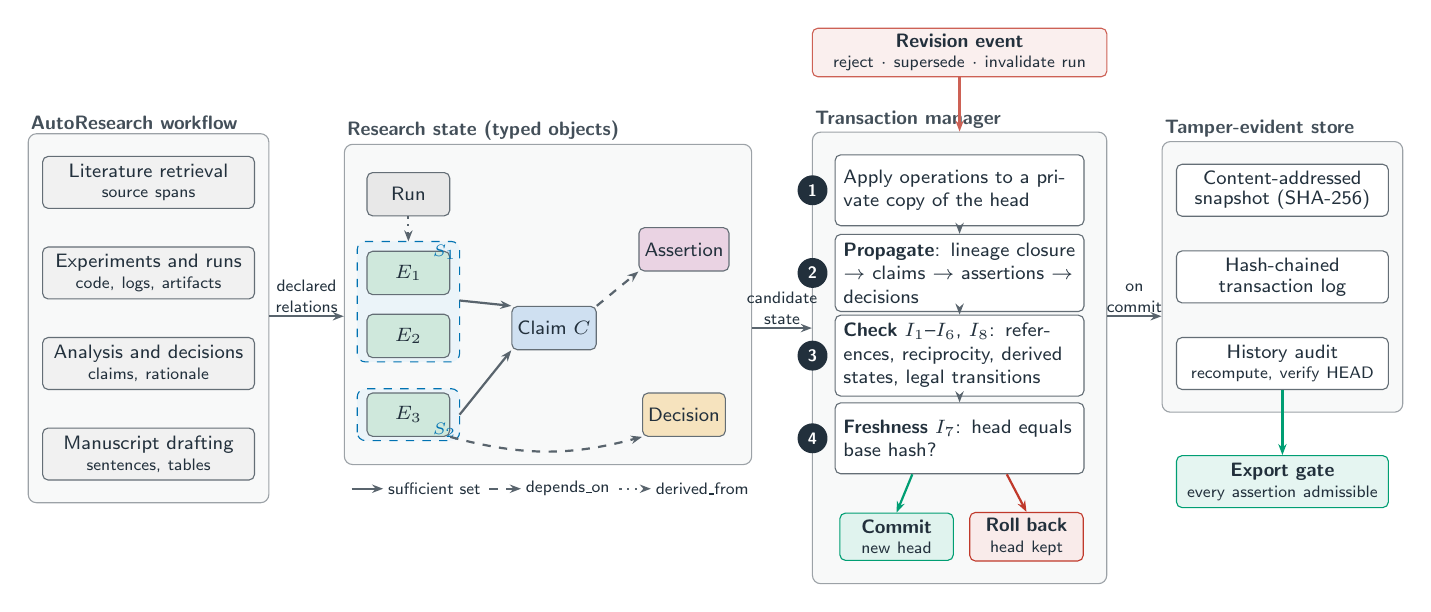
\begin{tikzpicture}[x=1cm,y=1cm]
% ---------------- A: AutoResearch workflow
\node[box, fill=cRun!60] (a1) at (1.45,4.7) {Literature retrieval\\[-1pt]{\tiny source spans}};
\node[box, fill=cRun!60] (a2) at (1.45,3.55) {Experiments and runs\\[-1pt]{\tiny code, logs, artifacts}};
\node[box, fill=cRun!60] (a3) at (1.45,2.4) {Analysis and decisions\\[-1pt]{\tiny claims, rationale}};
\node[box, fill=cRun!60] (a4) at (1.45,1.25) {Manuscript drafting\\[-1pt]{\tiny sentences, tables}};
\begin{scope}[on background layer]
\node[panel, fit=(a1)(a2)(a3)(a4), inner ysep=8pt] (PA) {};
\end{scope}
\node[ptitle] at (PA.north west) {AutoResearch workflow};

% ---------------- B: research state
\begin{scope}[shift={(4.1,0)}]
\path[draw=cGrp, dashed, rounded corners=3pt, fill=cGrp!8] (0.0,2.42) rectangle (1.3,3.95);
\path[draw=cGrp, dashed, rounded corners=3pt, fill=cGrp!8] (0.0,1.42) rectangle (1.3,2.08);
\node[obj, fill=cRun] (run) at (0.65,4.55) {Run};
\node[obj, fill=cEv] (e1) at (0.65,3.55) {$E_1$};
\node[obj, fill=cEv] (e2) at (0.65,2.75) {$E_2$};
\node[obj, fill=cEv] (e3) at (0.65,1.75) {$E_3$};
\node[obj, fill=cCl] (c) at (2.5,2.85) {Claim $C$};
\node[obj, fill=cAs] (a) at (4.15,3.85) {Assertion};
\node[obj, fill=cDe] (d) at (4.15,1.75) {Decision};
\node[font=\tiny\bfseries, text=cGrp, anchor=north east, inner sep=1pt] at (1.3,3.95) {$S_1$};
\node[font=\tiny\bfseries, text=cGrp, anchor=south east, inner sep=1pt] at (1.3,1.42) {$S_2$};
\draw[tarr] (run) -- (e1.north |- 0,3.95);
\draw[arr] (1.3,3.2) -- (c.north west);
\draw[arr] (1.3,1.75) -- (c.south west);
\draw[darr] (c.north east) -- (a.south west);
\draw[darr] (e3.south east) to[bend right=15] (d.south west);
\begin{scope}[on background layer]
\node[panel, fit=(run)(e3)(a)(d), inner ysep=10pt, inner xsep=8pt] (PB) {};
\end{scope}
\node[ptitle] at (PB.north west) {Research state (typed objects)};
\begin{scope}[shift={(PB.south west)}, xshift=0.1cm, yshift=-0.3cm]
\draw[arr] (0,0) -- (0.4,0); \node[anchor=west,font=\tiny, inner sep=1pt] at (0.42,0) {sufficient set};
\draw[darr] (1.75,0) -- (2.15,0); \node[anchor=west,font=\tiny, inner sep=1pt] at (2.17,0) {depends\_on};
\draw[tarr] (3.4,0) -- (3.8,0); \node[anchor=west,font=\tiny, inner sep=1pt] at (3.82,0) {derived\_from};
\end{scope}
\end{scope}

% ---------------- C: transaction manager
\begin{scope}[shift={(11.75,0)}]
\node[tstep] (t1) at (0,4.6) {Apply operations to a private copy of the head};
\node[tstep] (t2) at (0,3.55) {\textbf{Propagate}: lineage closure $\to$ claims $\to$ assertions $\to$ decisions};
\node[tstep] (t3) at (0,2.5) {\textbf{Check} $I_1$--$I_6$, $I_8$: references, reciprocity, derived states, legal transitions};
\node[tstep] (t4) at (0,1.45) {\textbf{Freshness} $I_7$: head equals base hash?};
\foreach \i/\n in {1/t1,2/t2,3/t3,4/t4}{\node[num] at ($(\n.west)+(-0.28,0)$) {\i};}
\draw[arr] (t1) -- (t2); \draw[arr] (t2) -- (t3); \draw[arr] (t3) -- (t4);
\node[draw=cOK, rounded corners=2pt, fill=cOK!12, text width=1.3cm, align=center, minimum height=0.6cm, inner sep=2pt] (ok) at (-0.8,0.2) {\textbf{Commit}\\[-1pt]{\tiny new head}};
\node[draw=cNo, rounded corners=2pt, fill=cNo!10, text width=1.3cm, align=center, minimum height=0.6cm, inner sep=2pt] (no) at (0.85,0.2) {\textbf{Roll back}\\[-1pt]{\tiny head kept}};
\draw[arr, draw=cOK] ([xshift=-0.6cm]t4.south) -- (ok.north);
\draw[arr, draw=cNo] ([xshift=0.6cm]t4.south) -- (no.north);
\begin{scope}[on background layer]
\node[panel, fit=(t1)(t4)(ok)(no), inner ysep=8pt, inner xsep=8pt] (PC) {};
\end{scope}
\node[ptitle] at (PC.north west) {Transaction manager};
\end{scope}

% ---------------- D: store and export
\begin{scope}[shift={(15.85,0)}]
\node[box] (s1n) at (0,4.6) {Content-addressed\\[-1pt]snapshot (SHA-256)};
\node[box] (s2n) at (0,3.5) {Hash-chained\\[-1pt]transaction log};
\node[box] (s3n) at (0,2.4) {History audit\\[-1pt]{\tiny recompute, verify HEAD}};
\node[box, fill=cOK!10, draw=cOK] (gate) at (0,0.9) {\textbf{Export gate}\\[-1pt]{\tiny every assertion admissible}};
\begin{scope}[on background layer]
\node[panel, fit=(s1n)(s3n), inner ysep=8pt] (PD) {};
\end{scope}
\node[ptitle] at (PD.north west) {Tamper-evident store};
\draw[arr, draw=cOK] (s3n.south) -- (gate.north);
\end{scope}

% ---------------- links between panels
\draw[arr] (PA.east |- 0,3.0) -- node[above,font=\tiny,align=center,inner sep=1pt]{declared\\relations} (PB.west |- 0,3.0);
\draw[arr] (PB.east |- 0,2.85) -- node[above,font=\tiny,align=center,inner sep=1pt]{candidate\\state} (PC.west |- 0,2.85);
\draw[arr] (PC.east |- 0,3.0) -- node[above,font=\tiny,align=center,inner sep=1pt]{on\\commit} (PD.west |- 0,3.0);
\node[draw=cNo!80, rounded corners=2pt, fill=cNo!8, text width=3.6cm, align=center, inner sep=2pt] (ev) at (11.75,6.35) {\textbf{Revision event}\\[-1pt]{\tiny reject $\cdot$ supersede $\cdot$ invalidate run}};
\draw[arr, draw=cNo!80] (ev.south) -- (PC.north |- ev.south) -- (t1.north |- PC.north);
\end{tikzpicture}
\end{document}
